% Changing book to article will make the footers match on each page,
% rather than alternate every other.
%
% Note that the article class does not have chapters.
\documentclass[letterpaper,10pt,twoside,twocolumn,openany]{book}

% Use babel or polyglossia to automatically redefine macros for terms
% Armor Class, Level, etc...
% Default output is in English; captions are located in lib/dndstring-captions.sty.
% If no captions exist for a language, English will be used.
%1. To load a language with babel:
%	\usepackage[<lang>]{babel}
%2. To load a language with polyglossia:
%	\usepackage{polyglossia}
%	\setdefaultlanguage{<lang>}
\usepackage[english]{babel}
%usepackage[italian]{babel}
% For further options (multilanguage documents, hypenations, language environments...)
% please refer to babel/polyglossia's documentation.

\usepackage[table]{xcolor}
\usepackage[utf8]{inputenc}
\usepackage{tikz}
\usetikzlibrary{shapes,arrows}
\usepackage{hang}
\usepackage{lipsum}
\usepackage{listings}

\usepackage{dnd}

\lstset{%
  basicstyle=\ttfamily,
  language=[LaTeX]{TeX},
}

\definecolor{desertsand}{rgb}{0.93, 0.79, 0.69}
\definecolor{darkterracotta}{rgb}{0.8, 0.31, 0.36}
% Define block styles
\tikzstyle{decision} = [diamond, draw, fill=desertsand!20, 
    text width=4.5em, text badly centered, node distance=3cm, inner sep=0pt]
\tikzstyle{block} = [rectangle, draw, fill=desertsand!20, 
    text width=8em, text centered, rounded corners, minimum height=4em]
\tikzstyle{line} = [draw, -latex']
\tikzstyle{cloud} = [draw, ellipse,fill=darkterracotta!20, node distance=3cm,
    minimum height=2em]


% Start document
\begin{document}

% Your content goes here

% Comment this out if you're using the article class.
\chapter{Design patterns for
\newline 
dungeons masters}

\section{Introduction}
I've been a dungeon master since I was 8 years old. I probably started with Heroquest and moved on to D\&D 3.5 when it came out. My father was a Dungeon Master of the first edition so I'm a proud second generation DM. During all this time, I like to think I developed some skills in this field; maybe it's something you have already seen in a youtube video, or in any another guide on how to DM. Maybe it's something you actually will find helpful, so I just want to share my experience, and if even just one person can benefit from it I'll be happy.

\subsection{What is a design pattern}
In software engineering, a software design pattern is a general, reusable solution to a commonly occurring problem within a given context in software design. It is not a finished design that can be transformed directly into source or machine code. It is a description or template for how to solve a problem that can be used in many different situations. Design patterns are formalized best practices that the programmer can use to solve common problems when designing an application or system\cite{wikipedia}.

A design pattern does not describe a specific situation or a specific context, but it's a well known and well tested approach to a general situation. I'm an IT guy and this term is really important in my job: the fact that some people out there decided to sit down and describe in a general way the best solution to a class of problem, really does make my life easier every day. As such, I decided to use the same approach, but with my Dungeon Master experience. We are not going to discuss settings or element here, but general situations I've seen happening over and over again and my suggestion on how to tackle them, improve the gaming skills of the whole party (yours included), and make sure everyone is enjoying the game.

\subsection{Version and License}
This document is an open source document version 1.0 is release on 06 December 2018, minor fix will be specified after the dot, major edit will change the version number.
This document is released under the MIT License.
\newline
Author: DangerBlack
\newline
Revision: xHawke

\section{Design pattern}

\subsection{The bending bamboo}
\subsubsection{The illusion of choice}
\textbf{Precondition:} Party reach a situation where one or more possible solution are available but one of the solution is clearly the correct one, the other one are completely absurd and gibberish nonsense. They keep failing those check that prevent you giving them information and they have some wrong idea about the world. \\
Another precondition is that they must not already know the map and the settings.
\newline
\begin{figure}[h]
\centering
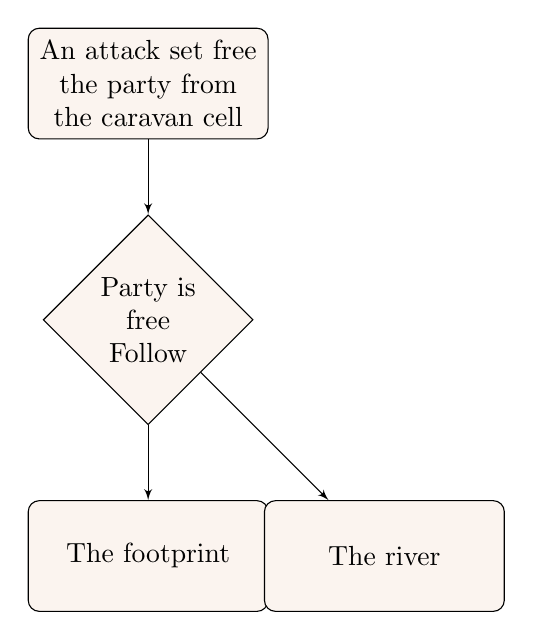
\begin{tikzpicture}[node distance = 2cm, auto]

\node [block] (init) {An attack set free the party from the caravan cell};
\node [decision, below of=init, node distance=3cm] (decide) {Party is free\\Follow};
\node [block, below of=decide, node distance=3cm] (option1) {The footprint};
\node [block, right of=option1, node distance=3cm] (option2) {The river};

\path [line] (init) -- (decide);
\path [line] (decide) -- (option1);
\path [line] (decide) -- (option2);
\end{tikzpicture}
\end{figure}

\noindent
\textbf{Description:} Whenever you are in such situation, you have probably done wrong the whole encounter, don't worry player are either bad at insight, there is only one thing you can do. You must nullify the outcome of their decision. The illusion of choice. Well you can force them to go to the right path or you can tell them more specifically underling with a strong mark some detail but player use to feel \textit{railroading} as a bad things, so I discourage you to use this approach instead just make them feel proud of their choice, swap the world, swap the entire universe if needed. Just collapse their decision three to what you want.

\subsection{The party splitter}
\subsubsection{How to force your player staying together}
\textbf{Precondition:} If you are not fully aware on how your player are at table you should consider to prevent a totally party split from the first session. Some people are just bad at this and keep pushing the game in other direction.

\begin{paperbox}{Example}
  Alduin: I know, I know that the world is going to and end, but I really care about my cow and my personal quest to be the greatest farmer of the last days. 
    So I'll wait the rest of the party here in the "Small and not well crafted" village where I can be the leader of a little industrial revolution.
\end{paperbox}

\noindent
\textbf{Description:} You shuld consider two option, first work on \textit{prepping}, second ask the player to leave, in the end this is absolutely the best decision but If you are friends in real life you should consider a better \textit{plot anchor}.
A plot anchor is a device that trigger your group together in a party, some example can be found in each manual I'll just proceed with few of them.

\begin{dndtable}[lX]
  \textbf{Name}         & \textbf{Description} \\
  Mark of chaos & A daemon have marked the player with a black mage they have to remove the mark or get killed.\\
  Forgotten Prophecy & The world is going to end and a prophecy address them by name each by each. \\
  Secret message & Heroes accidentally receive secret information about a cult or some terrible secrets now horde of enemies want them all dead.  
\end{dndtable}

\subsection{The ten hours' world building paradigm }
\subsubsection{Or how can you manage to roll again critical 1 on history check}
\textbf{Precondition:} Player keep failing check on key point situation, and you are no longer able to tell them important clue about their quest.
\newline
\noindent
\textbf{Description:} After you decide the name and the description of a forgotten sword named "Anduril, flame of the occident" with six page of the previous owner and the glorious feats that the iron have done in the past. Player fail to roll history check and you are no longer able to give them a single clue about those sword.
Well never mind my friend, time will come, just wait, put an NPC in another position enough far from the time line point and let him reveal freely some detail about that sword that the player keep using. The pattern is do not force a second check, just let the detail emerge while the player live the world. Some of the ten hour will probably never bubble on the top, but you already know that this is part of the game. This is a pattern to save a bad situation that you had to introduce, the following patter try to prevent this situation.


\subsection{Fate is a bitch}
\subsubsection{Do not let fate decide important aspect of what player know}
\textbf{Precondition:} *
\newline
\noindent
\textbf{Description:} If something is really really important do not let that a wrong dice destroy your work. Just let the player know, find and explore important aspect of the world.
Nobody want to be stuck in the same five by five room for six days just because the thief keep rolling 1 on find hidden door.
Well you may let the player check to find the door and even they fail, apply pattern \textit{The bending bamboo} and let a monster go out from the hidden door to attack the party.
Never frustrate your player, a bad game is not a game where everybody dies in an epic way, a bad game is when your player keep failing and keep blaming themselves for your ineptitude.

\subsection{Let the player play}
\subsubsection{Do not enter in the game}
\textbf{Precondition:} When you feel the urgency of acting or helping the party in a more straight way
\newline
\noindent
\textbf{Description:} You should never enter this way in game, no need for a Gandalf deus ex-machina NPC that solve the riddle for your players, or a overpowered Balrog's fighter. Well despite you can break this pattern for cinematic or tragedy purpose, you always carefully consider to not play a long lasting NPC near a party. If you do it, put in it on fallacy on purpose.
The forgotten identity, the brain damage, the obscure and dubious past, the will to go away from the party, or some other trait that let you turn it off when players want to "play" for real.

\subsection{Introduce a new player}
\subsubsection{When a friends ask you to play}
\textbf{Precondition:} Sometimes you are in a hidden cave, in the center of a maze or in some weird position but you really want to add a new player to the game. 
\newline
\noindent
\textbf{Description:} You can not add a party member without sense, and is hard to make it believable to your player, so pay attention:
\begin{itemize}
\item Do not force events
\item Avoid inserting new player
\item Determine quickly if player will keep playing with the party or if it just a one shot
\item Make it smooth
\end{itemize}

\begin{quotebox}
	We meet Clara in the goblin ruins she was kidnapped and bounded in a prison cell, we meet Marcus in the orks pit tied from head to toe, We meet Jhoanna in the mines and she was stunned by bandit.
\end{quotebox}

If this is your story you can see a pattern, you should break this pattern, try to randomize the process do not pick the easiest path. Dungeon master keep using the "tied up" solution because it helps creating a bond between player avoiding a possible \textit{Party splitter}. 

Here a easy to use table to randomize this pattern:
\begin{dndtable}[cX][DmgCoral]
  \textbf{d6} & \textbf{Item} \\
  1           & Tied up or Re-roll \\
  2           & Tavern, with info \\
  3           & Messenger\\
  4           & Need help from party \\
  6           & Save party assess \\
\end{dndtable}

\subsection{The Shy player}
\subsubsection{Helping a player feeling confident}
\textbf{Precondition:} If you play with a mixed party probably not all player will have the same screen time, some player love to interact and leads the group to their fate, on the other hand some player remain in the shadow for long time, probably bored.
\newline
\noindent
\textbf{Description:} Despite shy people do not like to be put in the center of attention you should consider by time to time to create condition where they are alone or unable to just call the other and have to fight a monster/ sneak a guard or / talk with a merchant about the cargo alone. Make them succeed and you will probably help them more than tree years of psychological help.

\subsection{Session Zero}
\subsubsection{Less is more}
\textbf{Precondition:} Creating character is really time consuming try not to start a game without building properly the characterization of each pg.
\newline
\noindent
\textbf{Description:} Some people in \textit{reddit} has started this new trend \textit{Session Zero}, a first session where player describe their character what they want from this game, what they like, and what they expect \cite{sessionzero}.
\begin{itemize}
\item  basic expectations for the overall campaign 
\item basic social etiquette (don't be mean, play nice with each other, no sexual assault of any kind in my games)
\item what their boundaries and triggers are
\item Figure out how the group wants to handle people missing one session.
\end{itemize}

\begin{quotebox}
	I accidentally play a rape scene in one of my game. You shouldn't. Even if is just a potential scene but player manage to interrupt it before. It may cause trouble to your player. Ask it in advance helps you define their boundaries. 
\end{quotebox}

\subsection{The rule of 3}
\subsubsection{Combat, Investigate, Interaction}
\textbf{Precondition:} Different player want different outcome from a session, you can have tree possible interaction in game, Combat, Investigate e Interaction. 
\newline
\noindent
\textbf{Description:} Most of d\&d is Combat, most of Call Of Cthulhu is Investigation, most of Vampire the masquerade or Fate is Interaction. Is not just the system that impose the interaction but also the genre that force the master in a specific way or another. You have to just not let the flow run, it's easy creating an never-ending linear dungeon full of monster and trap but hey, try to add a spicy investigation and a cool NPC interaction and your game will be wonderful.
I use the rule of 3, I split my session in three part and let player live a bite of each in each session or if a session is full Combat the next one could have a major part in investigation or interaction. Just try to variate and make it smooth for your player. 
\textbf{Corollary:} If your players (all of them) hate one of this interaction just change according to them. 

\subsection{I fucked up everything}
\subsubsection{Deus-ex-machina is not that bad}
\textbf{Precondition:} Sometimes one of your player make some choice beyond any redemption, they kill the daughter of the king or just go too far out of character to just switch back. I have a high priest who just become a smuggler. But after a while he feel very hard to play this character and he had no clue how to get back in line. He told me he want to quit or change character because of this! Red Flag!  
\newline
\noindent
\textbf{Description:} In impossible situation you have to use impossible tools to solve, just glide over the impossibility and make it happen. A god appear and talk with your priest and let him pay giving him a new holy mission. A magical phoenix save the princess making you possible to save players asses. I mean you can drastically change the world, you have the tools, do not forget it! DO NOT ABUSE IT! \textit{LET THE PLAYER PLAY}


\subsection{Magic shape your world}
\subsubsection{Use at your own risk}
\textbf{Precondition:} If you world-build your own universe be sure to take in account how magic work and it's limit. You have to ask yourself a lot of question!
\newline
\noindent
\textbf{Description:} I summarize most of the question in table \ref{tab:magic}, but speaking generally if you have some magical spell like fireball does it make sense that armies march in group? They will attack using phalanx or some other weird formation in order to minimize the loss. Wall in city make sense if people can't fly a better investment could be a school of magic or a flying infantry.
If your player can enter a random shop cast sleep on the cashier and steal 1000 pieces of gold your have probably failed in world building. 
Not because your world is bad, but because after 1000 years of evolution people take some precaution to this, they start killing magician bringer on spot from birth or maybe they start building city in places where magic do not work, like inside anti-magical field.
Magic are so common that each shop has a magician inside to check the costumer or better they have some amulet to stop level 1 magic at all?
Just plan ahead this kind of tricky situation in order to avoid lot of question in future. If you need more information just read Sanderson Laws of Magic\cite{magiclaw}. The three key element are Extrapolation, Interconnection and Streamlining.

\begin{itemize}
\item \textbf{Extrapolation:} Effects that a magic will have on a world.
\item \textbf{Interconnection:} Powers a character has seem like a coherent whole rather than separate abilities.
\item \textbf{Streamlining:} Combining pre-existing magics and powers is often better than adding new ones. Different culture reacting to a magic entirely differently than what has been shown so far.
\item \textbf{Balance(new):} This is a game not a book so try to make magic balanced.
\end{itemize}

\setthemecolor[PhbLightCyan]

\begin{table*}
\header{Magic precaution}
\begin{dndtable}[lX]
  \textbf{Aspect} & \textbf{Solution} \\
  Unlimited magic & Limit the number of spell per day, or make it risky throwing a spell \\
  Robbery using magic & People evolve ways to defend themselves, field of anti-magic penalty fee for abuser, magic linked with daemon \\
  Art of War & Change how war work with the presence of magic, tactics, sides, range, and proficiency.\\
  Magic diffusion & Is magic a common, uncommon or rare trait?\\
  Industrial Revolution & How does magic affect your industrial revolution, do people still use fire to forge weapons? Do people really still mine coal? Do oil is really a resources any more? The world changes just with a little spark of magic.\\
  Food and fire & Some magic create matter and this affect trade in some ways.\\
  Communication & Send message change the world, magic guild has unlimited power.\\
  Fast Travel & Does your world have something like the Sliph\cite{Slipth}?\\
  
\end{dndtable}
  \caption{Magic precaution aspect and solution}%
  \label{tab:magic}
\end{table*}

%\subsection{TITLE}
%\subsubsection{SUBTITLE}
%\textbf{Precondition:} PRECONDITION
%\newline
%\noindent
%\textbf{Description:} POST CONDITION


\tableofcontents

\bibliographystyle{unsrt}
\bibliography{bibliography}

\end{document}
